\documentclass[main.tex]{subfiles} % Subfile-Class


% ============================================================================== %
%                            Subfile document                                    %
% ============================================================================== %

\begin{document}

% Template

\subsubsection{Boardnetz}

Der folgende Abschnitt beschäftigt sich mit der Energieversorgung des
Pfadfinders. Wie die Evaluation der Energieversorgung ergeben hat, siehe
Anhang~\ref{appendix:Boardnetz}, wird der Roboter über einen 4S-LiPo mit
Energie versorgt. Die Ausgangsspannung von 14.4V wird auf dem selbst
entwickelten DC-PowerBoard mittels eines Abwärtsstellers auf 12V geregelt.
Dieses Board bietet ausserdem die Möglichkeit, über ein Netzteil in einem
Bereich von 12 bis 18 V versorgt zu werden und dabei den Akku selbsttätig zu
trennen. Dadurch ist der Roboter bei Entwicklungs- und Einrichtungsaufgaben
nicht zwingend auf die Energieversorgung via Batterie angewiesen, sondern kann
auch über ein Netzteil betrieben werden.

Die Batteriespannung und -strom werden über einen ADC überwacht und kann via
$I^2C$ vom Raspberry Pi ausgelesen werden.

Die Batterieschutzbeschaltung überwacht die Zellspannungen des LiPo-Akkus
jeweils getrennt und trennt die Batterie vom Gerät, falls eine der Zellen in
den Unterspannungsbereich gerät. Dieser Zustand wird über eine rot leuchtende
LED signalisiert. Die Zell-Balancierung ist nicht auf dem Pfadfinder selbst
umgesetzt. Für diesen Zweck ist ein Ladegerät aus dem Modellbaubereich gekauft,
welches die Zellen aktiv ausbalancieren kann.

Das Schema dieses PCB's, sowie sein Layout sind im Anhang beigefügt.
Abbildung~\ref{PowerBoard_Ansicht} zeigt eine 3D-Ansicht dieses PCB's.

\begin{figure}[H]
    \centering
    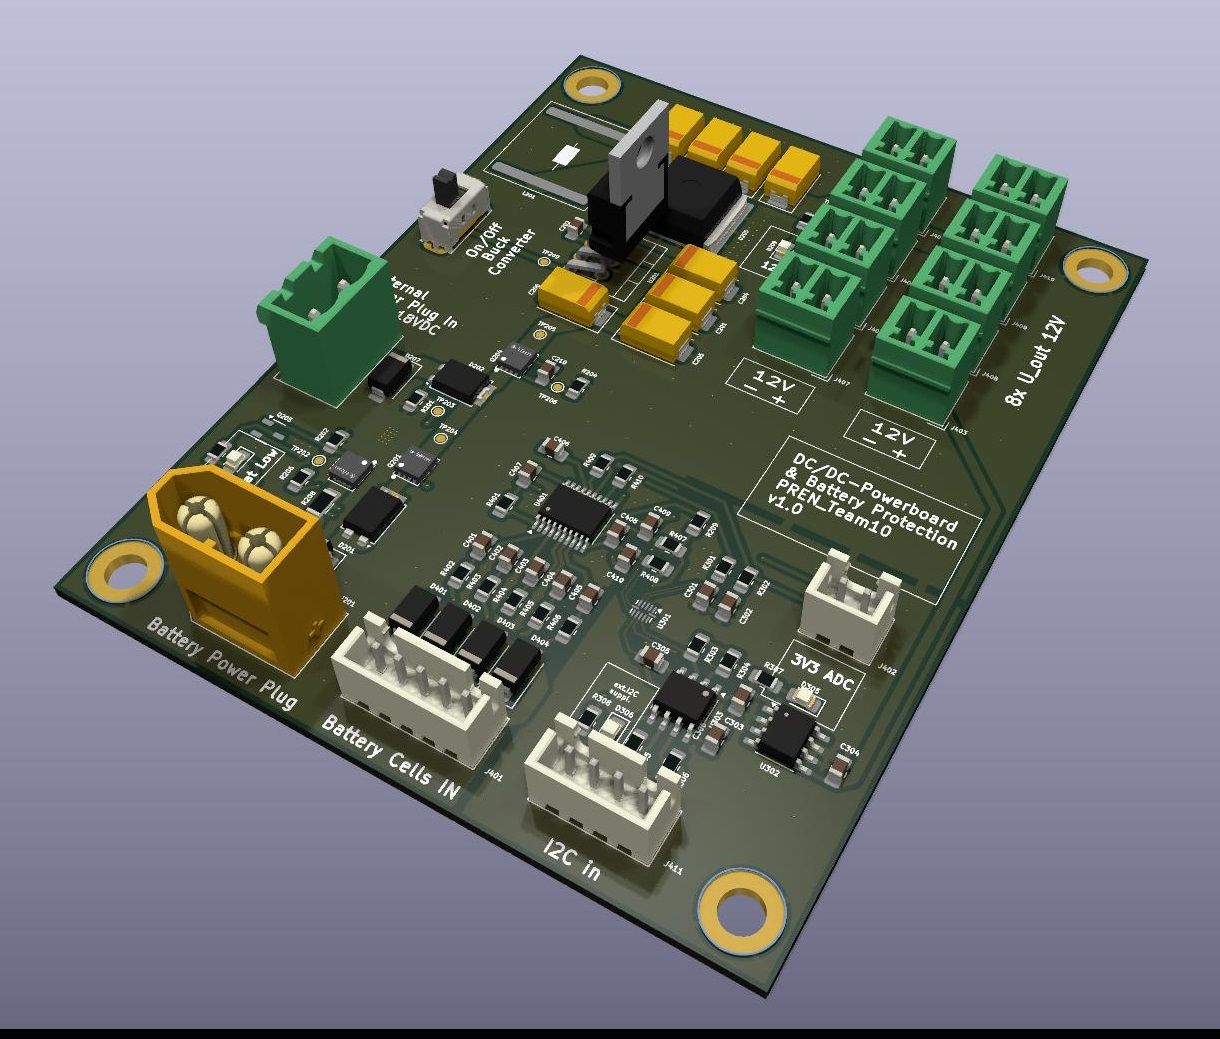
\includegraphics[width = 0.75\linewidth]{fig_Boardnetz/PowerDistributionBoard.jpg}
    \caption{Ansicht PowerBoard}~\label{PowerBoard_Ansicht}
\end{figure}

\paragraph{Boardnetz - Spannungsverteilung}
Jeder PCB wird über 12V mit Spannung versorgt. Auf den entsprechenden PCB's
werden die geregelten 12V zuerst über einen DC-DC Abwärtssteller auf $\approx$
6V heruntergebracht und dann über einen LDO auf 5V bzw. 3V3 aktiv gefiltert.
Dadurch wird verhindert, dass sich Spannungsspitzen oder Ripples durch zum
Beispiel die anlaufenden Motoren im gesamten System verteilen und andere
Elektronik stört. Für die LDO's wird ein PSSR angestrebt, welcher bei
entsprechenden Taktraten der Abwärtssteller eine angemessene Dämpfung von
mindestens $20dB$ aufweist. Das Blockschaltbild in
Abbildung~\ref{PowerBoard_Blockschaltbild} zeigt die Spannungsverteilung
konzeptionell.

\begin{figure}[H]
    \centering
    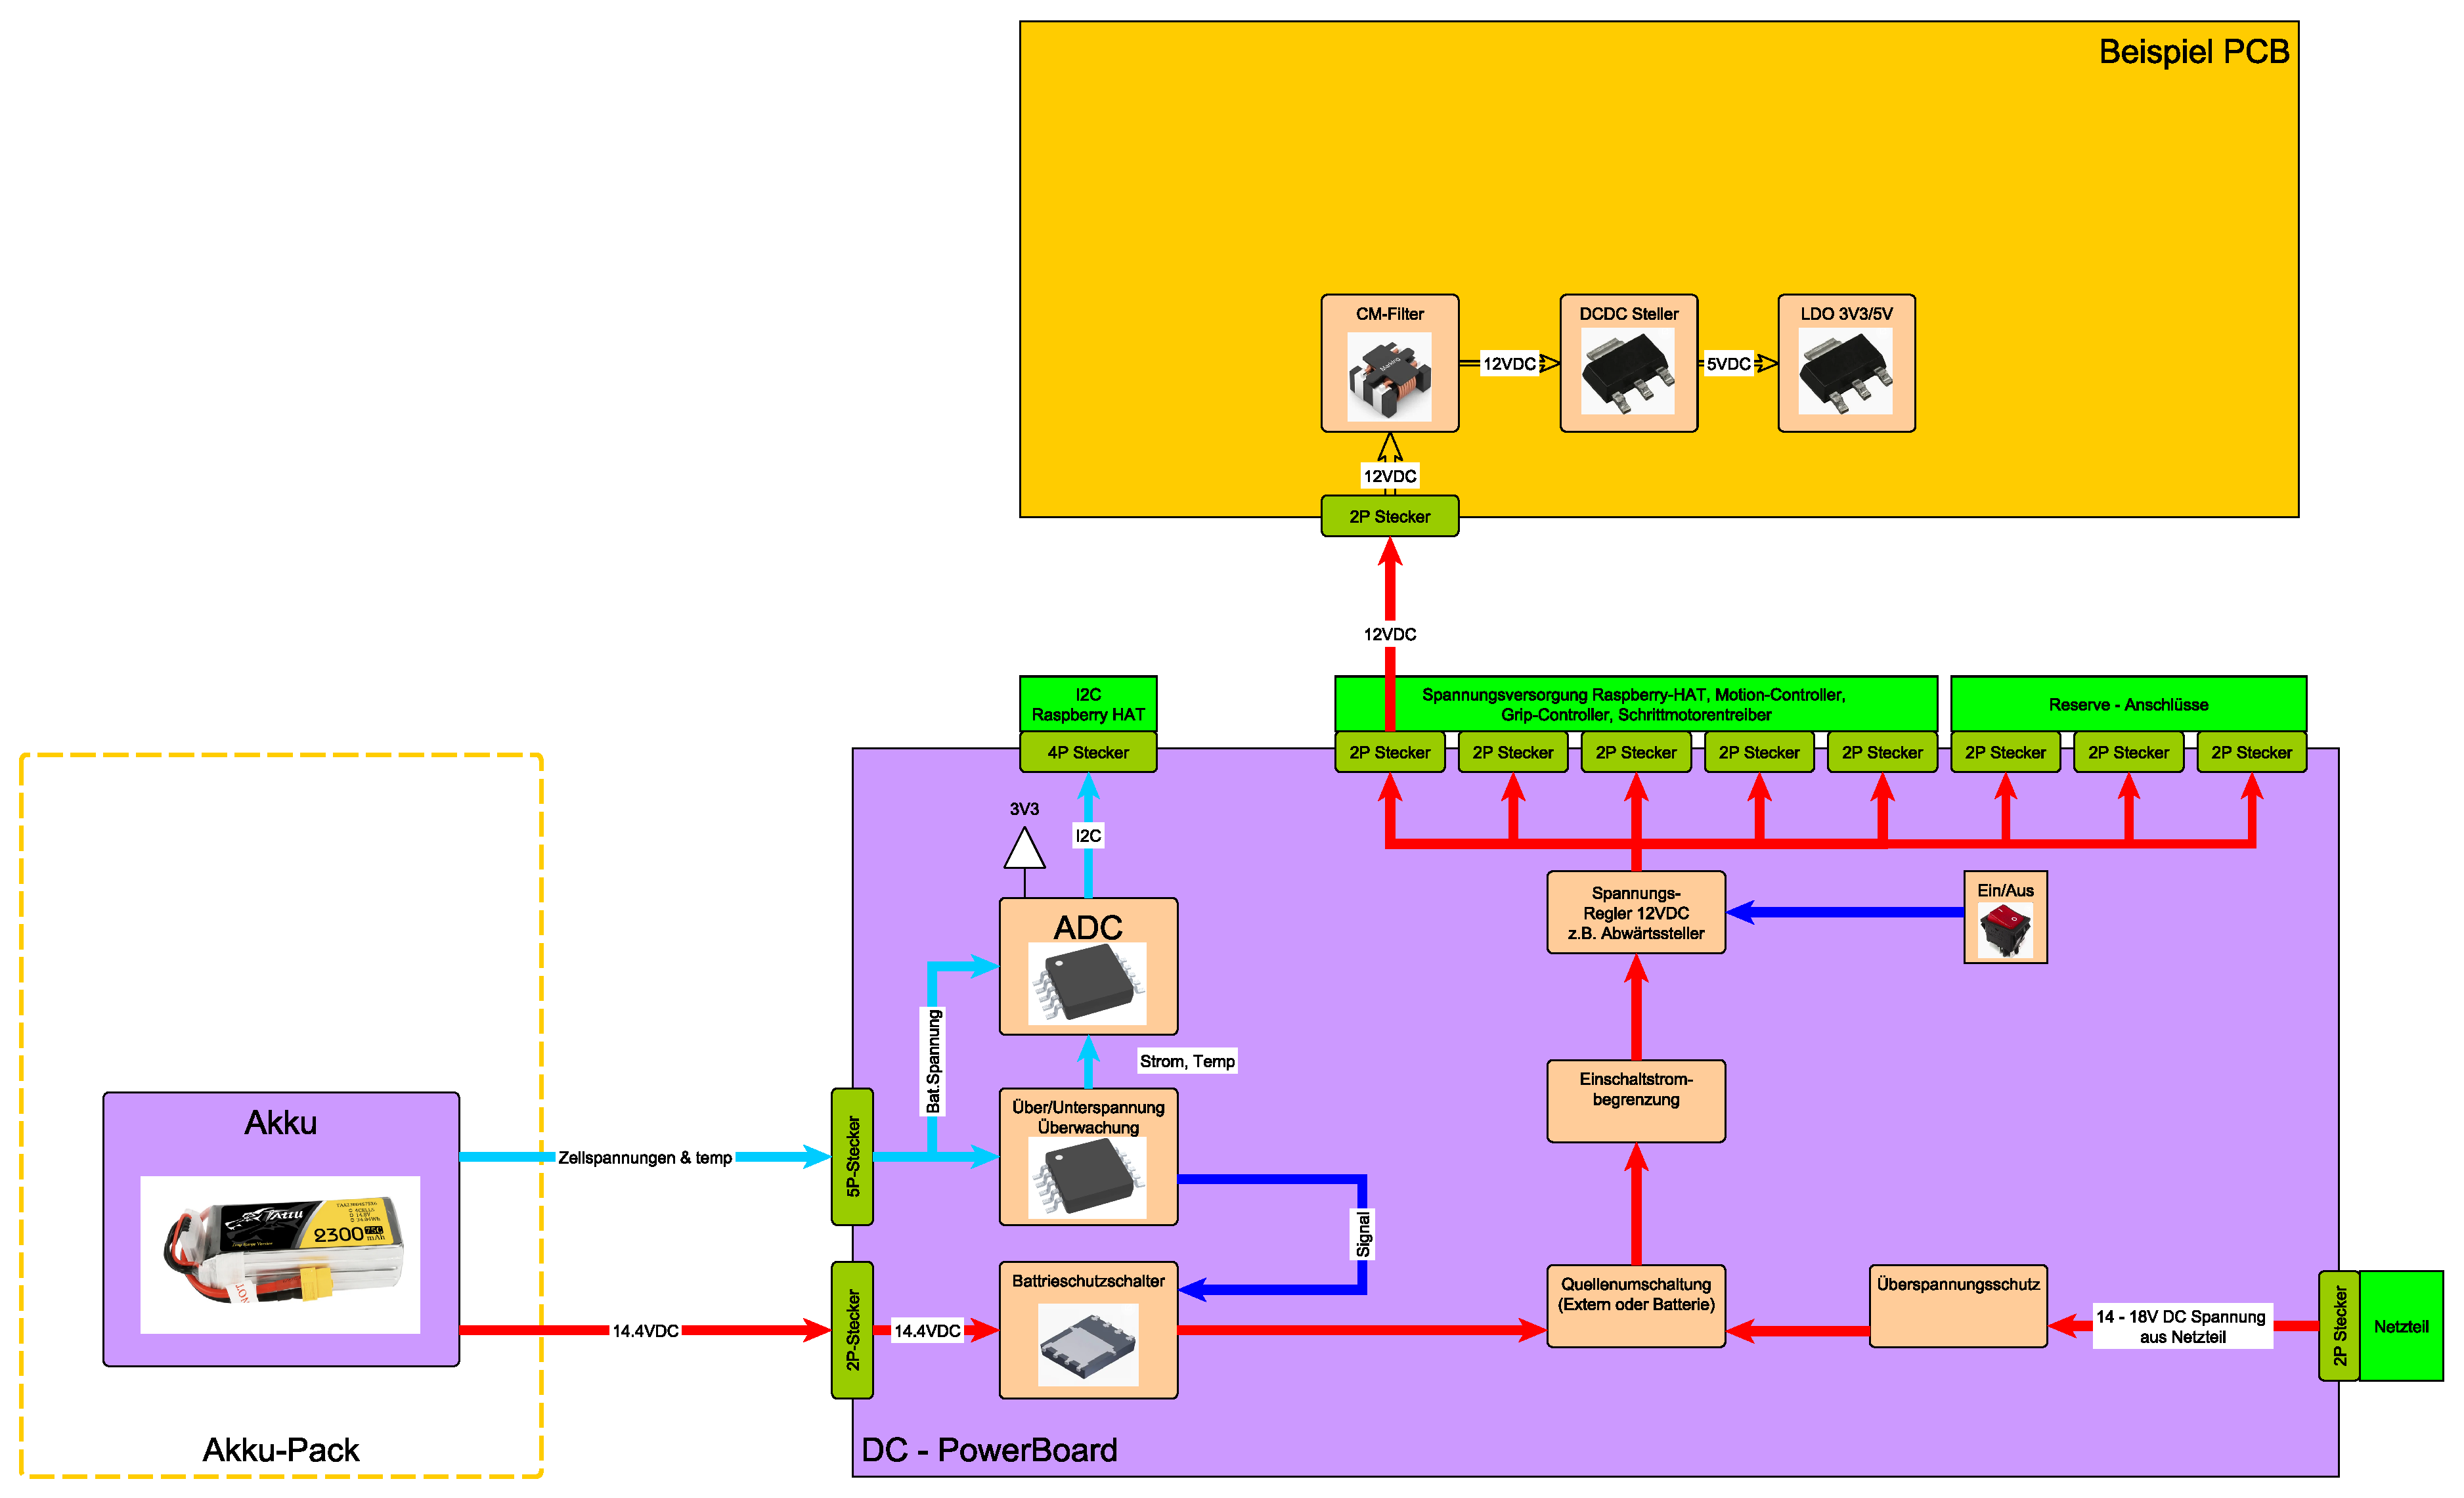
\includegraphics[width = 1\linewidth]{fig_Boardnetz/PowerBoard-Blockschaltbild.pdf}
    \caption{PowerBoard Blockschaltbild}~\label{PowerBoard_Blockschaltbild}
\end{figure}

\end{document}
